\documentclass[12px]{article}

\title{Lezione 24 Geometria I}
\date{2024-05-06}
\author{Federico De Sisti}

\usepackage{amsmath}
\usepackage{amsthm}
\usepackage{mdframed}
\usepackage{amssymb}
\usepackage{nicematrix}
\usepackage{amsfonts}
\usepackage{tcolorbox}
\tcbuselibrary{theorems}
\usepackage{xcolor}
\usepackage{cancel}

\newtheoremstyle{break}
  {1px}{1px}%
  {\itshape}{}%
  {\bfseries}{}%
  {\newline}{}%
\theoremstyle{break}
\newtheorem{theo}{Teorema}
\theoremstyle{break}
\newtheorem{lemma}{Lemma}
\theoremstyle{break}
\newtheorem{defin}{Definizione}
\theoremstyle{break}
\newtheorem{propo}{Proposizione}
\theoremstyle{break}
\newtheorem*{dimo}{Dimostrazione}
\theoremstyle{break}
\newtheorem*{es}{Esempio}

\newenvironment{dimo}
  {\begin{dimostrazione}}
  {\hfill\square\end{dimostrazione}}

\newenvironment{teo}
{\begin{mdframed}[linecolor=red, backgroundcolor=red!10]\begin{theo}}
  {\end{theo}\end{mdframed}}

\newenvironment{nome}
{\begin{mdframed}[linecolor=green, backgroundcolor=green!10]\begin{nomen}}
  {\end{nomen}\end{mdframed}}

\newenvironment{prop}
{\begin{mdframed}[linecolor=red, backgroundcolor=red!10]\begin{propo}}
  {\end{propo}\end{mdframed}}

\newenvironment{defi}
{\begin{mdframed}[linecolor=orange, backgroundcolor=orange!10]\begin{defin}}
  {\end{defin}\end{mdframed}}

\newenvironment{lemm}
{\begin{mdframed}[linecolor=red, backgroundcolor=red!10]\begin{lemma}}
  {\end{lemma}\end{mdframed}}

\newcommand{\icol}[1]{% inline column vector
  \left(\begin{smallmatrix}#1\end{smallmatrix}\right)%
}

\newcommand{\irow}[1]{% inline row vector
  \begin{smallmatrix}(#1)\end{smallmatrix}%
}

\newcommand{\matrice}[1]{% inline column vector
  \begin{pmatrix}#1\end{pmatrix}%
}

\newcommand{\C}{\mathbb{C}}
\newcommand{\K}{\mathbb{K}}
\newcommand{\R}{\mathbb{R}}


\begin{document}
	\maketitle
	\newpage
	\section{Spazi proiettivi e Antani}
	Servirebbe un'introduzione per tutto ciò, ma non sarà il Posta a darcela, la motivazione matematica è che la formula di Grassmann vale sempre (antani)
	\begin{defi}[Spazio Proiettivo]
		Sia $V$ uno spazio vettoriale di dimensione finita sul campo $\K$. Lo \textbf{spazio proiettivo} associato a  $V$ denominato con $\mathbb{P}(V)$ è l'insieme dei sottospazi $1 $-dimensionali di $V$ \\
		\[
			\K v \leftrightarrow [v] \storto{\storto{\leadsto}} \text{ punto di }\pro(v)
		.\] 
		$\dim V = 0 \ \ \ \mathbb{P}(V) = \emptyset$ \\
		$\dim V = 1 \ \ \ \mathbb{P}(V) = \{pt\}$ \\
		$\dim V = 2 \ \ \ \mathbb{P}(V)$ retta proiettiva\\
		$\dim V = 2 \ \ \ \mathbb{P}(V)$ piano proiettivo\\
		Quindi $\dim \mathbb{P}(V) = \dim V -1$\\
		Caso importante  $V = \K^{n+1}$\\
		 \[
			 \mathbb{P}(V) = \mathbb{P}^n(=\mathbb{P}^n(K))
		.\] 
	\end{defi}
	\textbf{Osservazione}\\
	1. Dati $v\in V\setminus \{0\}, \ \ \ \K v$ è un sottospazio $1 $-dimensionale, quindi esso dà luogo a un punto nello spazio proiettivo che denotiamo $[v]$\\
	2. La nozione di spazio proiettivo di $V$ può introdursi in modo equivalente tramite la seguente relazione d'equivalenza su $V\setminus \{0\}$
	 \[
		 v\sim w \Leftrightarrow \exists \lambda\in \K\setminus\{0\} \text{ t.c. } v= \lambda w
	.\] 
	Allora\\
	\begin{center}
	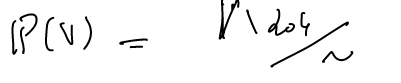
\includegraphics[scale=.5]{quoziente.png}\\
	\end{center}
	Riprendendo l'osservazione 1, nel caso $V=\K^{n+1}$
	 \[
		 (x_0,\ldots,x_n)\in\K^{n+1}\setminus\{0\} \leadsto [x_0\ldots,x_n]\in\mathbb{P}^n
	.\] 
	\[
		[x_0,\ldots,x_n]=[y_0,\ldots,y_n]
	.\] 
	\[ \Leftrightarrow\exists \lambda\in\K\setminus\{0\}:\ \ \ y_i= \lambda x_i, \ \ \ 0\leq i\leq n\]\\
	\begin{defi}
		Sia $\mathbb{P}=\mathbb{P}(V)$ ed $\{e_0,\ldots,e_n\}$ una base di $V$.\\
		Diciamo che $\{e_0,\ldots,e_n\}$ definisce un sistema di coordinate omogenee (o riferimento proiettivo) su $V$, denotato con $e_0,\ldots,e_n$
	\end{defi}
	Dato $v\in V\seminus\{0\}$
	 \[
	v= x_0e_0+\ldots +x_ne_n
	.\] 
	$\leadsto (x_0,\ldots,x_n)\in\K^{n+1}\setminus\{0\}$
	\[
		P[x_0,\ldots,x_n] \leftrightarrow P=[v]
	.\] 
	$x_0,\ldots,x_n$ si dicono coordinate omogenee di $v$
\\
Ad esempio, fissata la base $\{e_0,e_1,e_2\}$ in $\mathbb{P}^2$,\\
	$P[1,2,3]$ è il sottospazio $1 $-dim di $V$ generato da $e_0+2e_1+3e_2$\\
	\begin{nome}
		Fissato $e_0\ldots e_n$, i punti 
		\[
			F_0[1,0,\ldots,0] = [e_0],\ldots,F_n[0,\ldots,1]=[e_n] 
		.\] 
\\sono i punti fondamentali del riferimento\\
		$U[1,\ldots,1]$ punto unità del riferimento\\
		\textbf{Nota Bene}\\
		Poichè $[v] = [ \lambda v]$ risulta
		\[
		\lambda v = \lambda x_0e_0+\ldots+ \lambda x_n e_n
		.\] 
		quindi le coordinate omogenee sono determinate solo a meno di un fattore di proporzionalità non nullo
	\end{nome}
	\textbf{Osservazione}\\
	se $e_0,\ldots ,e_n$ è un riferimento proiettivo, anche  $(\mu e_0),\ldots,(\mu e_n), \ \ \mu\in\K\setminus\{0\}$ è un riferimento proiettivo e i punti hanno le stesse coordinate omogenee rispetto ai due riferimenti.\\
	\textbf{Quindi}\\
	consideriamo identici due riferimenti se definiti da basi proporzionali
	\[
	e_0,\ldots,e_n=(\mu e_0),\ldots,(\mu e_n)
	.\] 
	Un riferimento in $\mathbb{P}^n$ determinato dalla base canonica di $\K^{n+1}$ si dice riferimento standard. \\
	i punti fondamentali sono
	\[
		[1,0,\ldots,0],[0,1,\ldots,0],\ldots,[0,\ldots,0,1]
	.\] 
	\hline \ \\
	Dato $W\subset V$ sottospazio vettoriale possiamo considerare $\mathbb{P}(W)\leq \mathbb{P}(V)$\\
	$\mathbb{P}(W)$ è detto sottospazio proiettivo di $\mathbb{P}(V)$
	\[
		\dim\mathbb{P}(V)-\dim\mathbb{P}(W) = (\dim V-1) -(\dim W -1) = \dim V - \dim W
	.\] 

\begin{defi}
	Un iperpiano in $\pro^n$ è un sottospazio proiettivo di codimensione $1$
\end{defi}
Supponiamo che in $\pro^n$ sia fissato un riferimento $e_0,\ldots,e_n$ con coordinate omogenee $x_0,\ldots,x_n$
\[
	\circledast \ \ a_0x_0+a_1x_1+\ldots+a_nx_n=0 \ \ \icol{a_0\\\vdots\\a_n}\neq\icol{0\\\vdots\\0}
.\] 
Se leggiamo quest'equazione in $V$ è l'equazione cartesiana di un iperpiano vettoriale $H\subset V$\\
I punti di  $P=[v]\in \pro$ le cui coordinate omogenee verificano  $\circledast$ sono quelli tali che  $v\in H, \ \ v\neq 0$ quindi sono i punti di  $\pro(H)$ \\
\textbf{Nota bene}\\
Se $[x_0,\ldots, x_n] = [y_0,\ldots,y_n]$ e
\[
a_0x_0+\ldots+ a_nx_n=0
.\] 
allora anche $a_0y_0+\ldots+a_ny_n=0$ perché $[x_0,\ldots,x_n] = [y_0,\ldots,y_n]$ significa $y_i=\mu x_i \ \ \mu\in\K\setminus\{0\}$ e
 \[
a_0y_0+\ldots+a_ny_n=a_0\mu x_0+\ldots+a_n\mu x_n = \mu(a_0x_0+\ldots_a_nx_n)=0
.\] 
\  \hline \ \\
Iperpiani coordinati su $\pro^n$ (rispetto al riferimento standard)\[
	H_i=\{[x_0,\ldots,x_n]\in\pro^n|x_i=0\} \ \ 0\leq i\leq n
.\] 
Ad esempio, in $\pro^2,$   \begin{center}\begin{aligend}
	&H_0=\{x_0=0\}\\
	&H_1=\{x_1=0\}\\
	&H_2=\{x_2=0\}
\end{aligend}\end{center}\\
Più in generale consideriamo un sistema di $t$ equazioni omogenee\\
 \begin{cases}
	 &a_{10}x_0+\ldots a_{1n}x_n=0\\
	 &\ldots\\
	 &a_{t0}x_0+\ldots+a_{tn}x_n=0
 \end{cases}\\
 Se $W\subset V$ è il sottospazio definito dal sistema precedente, l'insieme di punti $P\in \pro$ le cui coordinate verificano il sistema è $\pro(W)$\\
 Sia $A=(a_{ij}) \ \ \ 1\leq i\leq t, 0\leq j\leq n$ e sia  $r=rk(A)$
  $\dim \pro(V)= \dim W -1=\dim V -r - 1 = \dim \pro(V) -r$
  Quindi  $\pro(W)$ ha codimensione $r$ su $\pro$\\
   \textbf{Intersezione}\\
   $A_1x = 0 \ \ \pro(W_1)$\\
   $A_2x=0 \ \ \pro(W_2)$ \\
   \begin{cases}
	&A_1x=0\\
	&A_2x=0
   \end{cases}
   In particolare $\pro(W_1)\cap\pro(W_2)= \emptyset \Leftrightarrow W_1\cap W_2 = \{0\}$
   \begin{defi}
   	$\pro(W_1),\pro(W_2)$ si dicono\\
	Incidenti se $\pro(W_1)\cap\pro(W_2)\neq\emptyset$\\
	Sghembi se $\pro(W_1)\cap\pro(W_2)=\emptyset$
   \end{defi}
   \textbf{Osservazione}\\
   La formula si generalizza in 
   \[
	   \bigcap_{i\in I}\pro(W_i) = \pro\left(\bigcap_{i\in I }W_i\right)
   .\] 
   \begin{defi}
   	Se $\emptyset\neq J\subset \pro$, il sottospazio proiettivo generato da  $J$ è 
	\[
		L(J)=\bigcap_{\pro(W)\supseteq J}\pro(W)
	.\] 
	con $W$ sottospazio di $V$
   \end{defi}
   \textbf{Caso speciale}\\
   $J=\{p_1,\ldots, p_t\}$. Scriveremo in tal caso $L(p_1,\ldots,p_y)$ Notiamo che se
   \[
	   p_1=[v_1],\ldots,p_t=[v_t]
   .\] 
   \[
   L(p_1,\ldots,p_t)=\pro(<v_1,\ldots,v_t>)
   .\] 
   In particolare \\
   $\dim(L(p_1,\ldots,p_t))\leq t-1$ 
   \begin{defi}
   	$p_1,\ldots,p_t$ si dicono linearmente indipendenti se 
	\[
	\dim(L(p_1,\ldots, p_t))=t-1
	.\] 
   \end{defi}
   \textbf{Esempio}\\
   $p_1,p_2$ sono indipendenti $ \Leftrightarrow$ sono distinti \\
   $p_1,p_2,p_3$ sono indipendenti $ \Leftrightarrow$ non sono allineati
   \newpage
   \begin{defi}
   	$p_1,\ldots,p_t$ in $\pro=\pro(V)$, $\dim(V)=n+1$ si dicono in posizione generale se\\
	$\circ$ sono linearmente indipendenti $(t\leq n+1)$\\
	 $\circ$ se $t>n+1$ e $n+1$ tra essi, comunque scelti, sono linearmente indipendenti
   \end{defi}
\textbf{Esempio} su $\pro^2$\\
	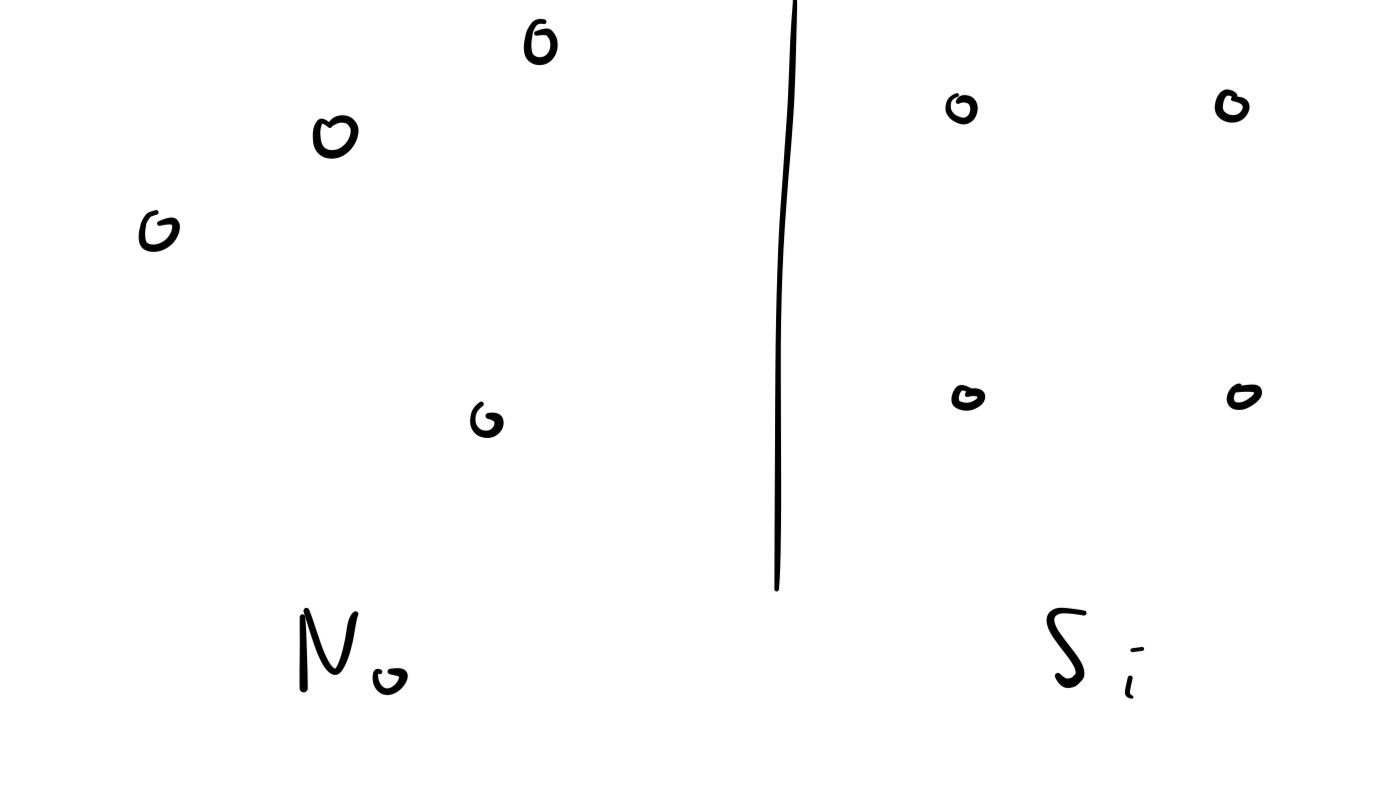
\includegraphics[scale=0.20]{pos_gen.jpeg}
	\subsection{Equazioni parametriche di un sottospazio}
	$k+1$ punti linearmente indipendenti $[v_0],\ldots,[v_n]$ in un sottospazio proiettivo $S$ di dimensione $k$.\\
	Per ogni $P\in S$, 
	\[
		P = [\lambda_0v_0+ \lambda_1v_1+\ldots+ \lambda_k v_k]
	.\] 
	Fissiamo ora un riferimento $e_0,\ldots,e_n$ su $\pro$\\
Allora se $v_i$ ha coordinate $(p_{i0},\ldots,p_{in})^t$ rispetto a $\{e_0,\ldots,e_n\}$ e $P = P[x_0,\ldots,x_n]$ si ha
\begin{center}
\begin{cases}
	x_0 = \lambda_0 p_{00}+ \lambda_1p_{10}+\ldots+ \lambda_k p_{k0}\\
	x_1 = \lambda_0 p_{01}+ \lambda_1p_{11}+\ldots+ \lambda_k p_{k1}\\
	\vdots\\

	x_n = \lambda_0 p_{0n}+ \lambda_1p_{1n}+\ldots+ \lambda_k p_{kn}\\
\end{cases}\end{center}
\textbf{Caso importante}: rette $[v_0],[v_1]$\\
\begin{center}\begin{cases}
	x_0 = \lambda_0 p_{00}+ \lambda_1 p_{10}\\
	x_0 = \lambda_0 p_{01}+ \lambda_1 p_{11}\\
	\vdots\\
	x_0 = \lambda_0 p_{0n}+ \lambda_1 p_{1n}\\
\end{cases}\end{center}\\
\ \\ \hline \ \\
$\pro$ piano proiettivo, $r$ retta per $P[p_0,p_1,2],Q[q_0,q_1,q_2]$ $r$ è un iperpiano in $\pro$ 
\[
	\det\matrice{x_0&x_1&x_2\\p_0&p_1&p_2\\q_0&q_1&q_2}=0
.\] 
\textbf{Esercizio} Se in $\pro^3$ sono dati punti non allineati 
\[
	P[p_0,p_1,p_2,p_3],Q[q_0,q_1,q_2,q_3],R[r_0,r_1,r_2,r_3]
.\] 
l'equazione del piano per $P,Q,E$ è
 \[
	 \det\matrice{x_0&x_1&x_2&x_3\\p_0&p_1&p_2&p_3\\q_0&q_1&q_2&q_3\\r_0&r_1&r_2&r_3}=0
.\] 
\textbf{Esempio} Retta in $\pro^2(\C)$ per $[-1,1,1],[1,3,2i]$
\[
	\det\matrice{x_0&x_1&x_2\\-1&1&1\\1&3&2i}=0
.\] 
$\circ$ Verificare che i punti $A=[1,2,2], B=[3,1,4],C = [\ldots]$ di  $\pro^2(\R)$ sono allineati e scrivere un'equazione ella retta che li contiene
\[
	\det\matrice{x_0&x_1&x_2\\1&2&2\\3&1&4}=0
.\] 
$\circ$ Verificare che le rette per $\pro(\C)$ \\
\begin{aligned}
	&ix_1-x_2+3ix_0=0\\
	&x_0+x_1-ix_2=0\\
	&5x_0 + x_1 + 3ix_2
\end{aligned}\\
hanno intersezione non vuota (basta verificare che il determinante sia nullo)
\[
	A=\matrice{3i&i&-1\\1&1&-i\\5&1&3i}
.\] 
$\det A = 0$
\ \\ \hline \ \\
Siano $S_1= \pro(W_1), S_2=\pro(W_2)$ due sottospazi proiettivi
\[
	L(S_1\cup S_2) \text{ è detto sottospazio somma}
.\] 
\[
L(S_1,S_2) = P(W_1+W_2)
.\] 
Infatti, se $\pro(W)\supset S_1\cup S_2$, allora contiene $\pro(W_1+W_2)$ perché $W$ deve contenere sia $W_1$ che $W_2$ \\
D'altra parte, $W_1+W_2\supseteq W_1, \ \ W_1+W_2\supseteq W_2$\\
quindi$
\begin{aligend}
	\hspace{20px}&\pro(W_1+W_2)\supseteq P(W_1)=S_1\\
	&\pro(W_1+W_2)\supseteq P(W_2)=S_2
\end{aligend} 
\Rightarrow \supseteq L(S_1,S_2)$
\begin{teo}[Forumla di Grassmann proiettiva]
\[
\dim L(S_1,S_2)=\dim S_1+\dim S_2 - \dim S_1\cap S_2
.\] 
($S1,S_2$ sottospazi proiettivi di $\pro(V)$
\end{teo}
\begin{dimo}
	La dimostrazione segue subito dalla formula di Grassmann vettoriale
	\[
	\dim(W_1+W_2) = \dim W_1 + \dim W_2 - \dim W_1\cap W_2
	.\] 
	$\dim L(S_1,S_2) - 1 = \dim S + 1 + \dim S_2 + 1 - (\dim S1\cap S_2 + 2)$
\end{dimo}
\textbf{Osservazione}\\
Poiché $\dim L(S_1,S_2)\leq \dim \pro$, risulta dalla formula di Grassmann
\[
	\dim S_1\cap S_2 \geq \dim S_1 + \dim S_2 - \dim \pro
.\] 
In particolare
\[
	\dim S_1 + \dim S_2 \geq \dim \pro \Rightarrow S_1,S_2 \text{ sono incidenti}
.\] 
(Infatti $\dim S_1\cap S_2\geq 0 \Leftrightarrow S_1\geq S_2 \neq \emptyset)$ 
\begin{coro}
	1. In un piano proiettivo due rette si intersecano\\
	2. In uno spazio proiettivo di dimensione 3 una retta e un piano si intersecano e due piani distinti si intersecano in una retta
\end{coro}
\end{document}
